% !TeX spellcheck = it_IT
\documentclass[12pt, italian]{article}
\usepackage[utf8]{inputenc}
\usepackage {graphicx}
\usepackage{hyperref} 
\usepackage{float}

\title{\textbf{THO\\Treasure Hunt Organizer}}
\author{
	Caselli, Ashley\\
	\texttt{ashley.caselli@studio.unibo.it}
	\and
	Mambelli, Giacomo\\
	\texttt{giacomo.mambelli@studio.unibo.it}
	\and
	Tassinari, Francesca\\
	\texttt{francesc.tassinari10@studio.unibo.it}
	\and
	Vattimo, Carmine\\
	\texttt{carmine.vattimo@studio.unibo.it}
}
\date{\today}

\begin{document}
\maketitle
\newpage
\tableofcontents
\newpage

\section{Introduction}
% descrizione anche sommaria di cosa il sistema implementato realizza
% This document contains the final work of PPS course. The goal has been
% Il focus di tale progetto è, oltre all'effettivo sviluppo del sistema, il processo adottato per lo sviluppo in team, mettendo in pratica al meglio possibile ciò che è stato ampiamente studiato nel corso.
This document contains the final work of PPS course. The focus of this project is, in addition to realised the system, as we have learned and studied in the couse is work in a team and divided the task.
The goal has been the implementation of a software system, using good technics of implementation, team organization and work flow and apply in the best way possible the teachings of the PPS course.\\
THO (Treasure Hunt Organizer) is a software system that helps in the organization and during the play time of treasure hunts.
The system provides a desktop software to the organizer of the hunt and a web application designed for the players.\\
The desktop module is an application aimed to make as simple as possible the organization of a treasure hunt. This purpose is actualized by a minimal user interface that allows to create, modify and manage a hunt with its points of interest (POI).\\
The players which walk around during the game and need clues and information to make them able to win are helped by the web application. This app provides a map showing the position of the device and purpose to the user quiz and clue useful to reach all the points of interest of the running treasure hunt.\\
All the data of the hunts are saved on a database hosted by a server that also has the task of managing the communication.

\section{Processo di sviluppo software}
\section{Metodologia di sviluppo}
Inizialmente i membri del progetto "THO" hanno individuato la figura del Product Owner in Carmine Vattimo come autore dell'idea proposta. Per lo sviluppo del sistema THO si è adottato un approccio Agile di schedulazione divisione e verifica dei task adottando come modalità di sviluppo Scrum. 
\\ Inizialmente abbiamo proceduto ad analizzare l'idea iniziale del progetto come segue:
\begin{itemize}
	\item Individuazioni specifiche di base;
	\item Individuazione entità da sviluppare;
	\item Scelta di quale broker per lo scambio di messaggi utilizzare;
	\item Scelta del database;
	\item Scelta dei linguaggi di programmazione desktop e mobile.
\end{itemize}

Al termine di questa fase abbiamo poi pianificato su Trello i 5 sprint da 20 ore, in cui a fine di ognuno di essi, abbiamo fatto una sprint review.\\Dopo aver svolto l'analisi del problema abbiamo creato il Product Backlog composto da varie user story, suddivise nei 5 sprint in ordine di priorità. \\

{\ [immagine del product backlog]}\\

Le user story sono poi state ampliate in vari task, che durante le sprint review ogni membro del team doveva assegnarsi per poi portare a termine. \\Una sprint review iniziava raccontandoci e spiegandoci cosa, uno o più membri del gruppo, avevano fatto durante i giorni trascorsi. A fine di ogni sprint review si valutava il lavoro compiuto, si creava nuovi task, ci si divideva i nuovi compiti e si stabiliva, approssimativamente, il tempo pensato per lo svolgimento dei nuovi task assegnati. Durante queste sprint review è stato possibile monitorare l'avanzamento del progetto. Inizialmente abbiamo avuto qualche difficoltà a utilizzare la modalità di sviluppo Scrum, perchè non avevamo chiaro come si costruiva e come funzionava un Product Backlog. Qualche difficoltà durante l'avvio del progetto l'abbiamo riscontrata anche nello stimare i tempi per lo svolgimento di ogni singolo task, non sapevamo come calcolare le ore e come metterle nel Product Backlog. E' stato veramente un lavoro di squadra dove ognuno metteva in campo il proprio sapere. A volte alcuni task venivano anche svolti insieme fra alcuni membri del progetto affinchè il know-how di ogni componente potesse aumentare grazie all'altra persona.
\section{Modalità di sviluppo}
\begin{itemize}
	\item \textbf{Scrum} utilizzato per la gestione del ciclo di sviluppo del progetto.
\end{itemize}
\section{Strumenti di sviluppo}
\begin{itemize}
	\item \textbf{Trello} utilizzato come bacheca per la divisione dei compiti;
	\item \textbf{Gradle} utilizzato come sistema per lo sviluppo del progetto;
	\item \textbf{IntelliJ IDEA} ambiente di sviluppo;
	\item \textbf{Git} utilizzato per il controllo delle versioni;
	\item \textbf{GitHub} utilizzato come repository;
	\item \textbf{Travis CI} utilizzato come build e test del progetto.
\end{itemize}

\section{Requisiti}
\section{Requisiti funzionali}
THO è un sistema distribuito con cui è possibile organizzare e giocare a cacce al tesoro. Utilizzando l'approccio Agile nel primo sprint abbiamo investito molte ore proprio nel raffinamento dei requisiti, ovvero abbiamo pensato come doveva funzionare il progetto e definire i compiti delle varie entità. In questo modo abbiamo evidenziato i requisiti funzionali:
\begin{itemize}
	\item \textbf{Lato Organizzatore} 
	\begin{enumerate}
		\item Creare una nuova caccia al tesoro.
			\begin{enumerate}
				\item [a.] Inserire il nome della nuova caccia al tesoro.
				\item [b.] Inserire la data di inzio della nuova caccia al tesoro.
				\item [c.] Inserire l'ora di inzio della nuova caccia al tesoro.
				\item [d.] Inserire nella mappa il luogo di svolgimento della caccia al tesoro.
				\item [e.] Inserire nella mappa i punti di interesse che dovranno essere ragginti dai giocatori.
				\item [f.] Nei punti di interesse aggiungere anche il quiz da risolvere e quando l'indizio per il prossimo punto di interesse.
				\item [g.] Cancellare/aggiungere dei punti di interesse con rispettivi indizi e quiz.
				\item [h.] Visualizzare i punti di interesse già creati in un'elenco.
				\item [i.] Far partire la caccia al tesoro oppure stopparla.
			\end{enumerate}
		\item Caricare una caccia al tesoro già creata.
		\begin{enumerate}
			\item [a.] Visualizzare il codice della caccia al tesoro.
			\item [b.] Visualizzare i punti di interesse già creati in un'elenco.
			\item [c.] Cancellare/aggiungere dei punti di interesse con rispettivi indizzi e quiz.
			\item [d.] Aprire le iscrizioni a una caccia al tesoro e avviarla.
		\end{enumerate}
		\item Cancellare Una caccia al tesoro già creata.
	\end{enumerate}
	\item \textbf{Lato Giocatore}
		\begin{enumerate}
			\item Creare un account.
			\begin{enumerate}
				\item [a.] Creare il nome del gruppo.
				\item [b.] Creare la password del gruppo.
				\item [c.] Confermare la nuova password del gruppo.
			\end{enumerate}
			\item Accedere tramite login del gruppo.
			\begin{enumerate}
				\item [a.] Visualizzare la lista delle cacce al tesoro con iscrizioni aperte.
				\item [b.] Scelta di una caccia al tesoro.
				\item [c.] Visualizzare la mappa della caccia al tesoro.
				\item [d.] Riceve i quiz.
				\item [e.] Ricevere gli indizi per raggiungere la nuova caccia al tesoro.
			\end{enumerate}
		\end{enumerate} 
	\item \textbf{Lato Server}
		\begin{enumerate}
			\item Il server deve gestire le operazioni sul database.
			\item Il server deve gestire i messaggi in ingresso e inviare le risposte.
		\end{enumerate}
\end{itemize}


\section{Requisiti non funzionali}
I requisiti non funzionali sono stati identificati come segue:
\begin{itemize}
	\item Sia la parte desktop e l'applicazione mobile devono essere user-friendly.
	\item La creazione di una nuova caccia al tesoro, con i rispettivi punti di interesse, quiz e indizi devono essere salvati nel database.
	\item Quando un giocatore arriva a un punto di interesse gli deve arrivare il quiz, se risponde correttamente a un quiz gli deve essere mandato l'indizio del punto di interesse successivo.
	\item Quando un giocatore finisce la caccia al tesoro gli verrà notificato al suo dispositivo e verrà notificato anche all'organizzatore.
\end{itemize}
%Rabbit Usage: As a possible counter-effect is that adding RabbitMQ in the middle, you will add some latency to the solution. However you have the possibility to gain in terms of reliability, flexibility, scalability,...


\section{Design architetturale}
\subsection{Desktop}
\subsubsection{Model-View-Controller}
\subsubsection{Observer}
\subsection{App Mobile}
\subsubsection{App Ibrida}
\subsection{Server}
\subsubsection{Middleware}
\subsubsection{Data Access Layer}
\subsubsection{Database}

\section{Design di dettaglio}
L'applicazione THO, ha lo scopo di gestire le cacce al tesoro create da un organizzatore che dopo aver scelto una location/città in cui svolgere la gara, aver scelto i punti di interesse, aver inserito i relativi indovinelli nei POI e aver fatto iscrivere i team a una caccia ben specifica potrà far partire la gara.
\\Abbiamo deciso che questa applicazione abbia una visione desktop e una mobile.
L’idea di base prevede due macro-sistemi:
\begin{itemize}
	\item L'organizzatore
	\item I giocatori partecipanti alla caccia al tesoro
\end{itemize}
\subsection{Organizzatore}
L’organizzazione di una caccia al tesoro viene fatta tramite un’applicazione desktop che permette all'organizzatore di scegliere una città/location per il gioco tramite una mappa. Attraverso tale mappa ha la possibilità di impostare i punti di interesse che corrisponderanno alle varie tappe del gioco. Ad ogni punto di interesse è associato un mini gioco/indovinello che sarà creato e poi fornito ad ogni team che durante la caccia raggiungerà tale punto. La corretta risoluzione del quiz consentirà al team di avanzare nel gioco.\\
L'organizzatore, a gioco avviato, ha la possibilità di controllarne l'andamento ed eventualmente di dare indicazioni in tempo reale ai team per aiutarli ad arrivare al successivo punto di interesse oppure di inviare un messaggio di vincita della caccia al tesoro da parte di un team.\\

L’organizzatore di una caccia al tesoro avrà a disposizione una interfaccia grafica che gli consenta di creare, modificare e gestire le varie fasi di gioco.\\
Potrà creare una nuova caccia al tesoro scegliendo un nome che la renda riconoscibile, una data ed un orario di svolgimento.\\
L’organizzatore potrà chiudere l’applicazione desktop senza perdere la caccia al tesoro creata, potendola utilizzare, modificare ed avviare in seguito.\\
A sua disposizione ci sarà l’elenco delle cacce al tesoro precedentemente create e non ancora giocate. Potrà selezionarne una ed aprirla, cioè modificarla.\\
L’organizzatore potrà scegliere una città, impostandola come zona principale di svolgimento dell’evento di gioco.\\
Visualizzerà una mappa all’interno dell’interfaccia dove poter inserire, cliccando, tutti i POI della caccia al tesoro.\\
Potrà, al momento della creazione di un POI, specificare un indizio che il giocatore potrà visualizzare e sfruttare per raggiungere il POI stesso.\\
Potrà anche specificare un quiz, con rispettiva risposta, al quale il giocatore dovrà rispondere per poter visualizzare l’indizio precedentemente inserito.\\
L’organizzatore potrà eliminare i POI precedentemente creati.\\
Potrà richiedere un codice numerico da diffondere ai partecipanti, che lo useranno come chiave di accesso per l’iscrizione alla caccia al tesoro.\\
L’organizzatore avrà la possibilità di decidere il momento in cui aprire le iscrizioni alla caccia al tesoro cliccando su in apposito tasto.\\
Analogamente potrà chiudere le iscrizioni.\\
L’organizzatore non potrà modificare la caccia al tesoro se è già in svolgimento, cioè se ne ha già aperto le iscrizioni.\\


\subsection{Giocatore}
Il sistema lato giocatori consiste nello sviluppo di un'applicazione mobile, che attraverso il GPS li colloca sulla mappa di gioco e permette loro di essere avvisati nel momento in cui raggiungono un determinato punto di interesse. Il raggiungimento di un punto di interesse permetterà loro di ricevere il quiz associato a tale punto e, successivamente alla corretta risoluzione del quiz, anche il nuovo indizio che gli consentirà di procedere nel gioco.
\subsection{Desktop}
L'applicazione desktop può essere utilizzata solo dall'organizzatore, 
\subsection{App Mobile}
L'applicazione mobile può essere utilizzata da tutti i giocatori che si sono loggati in una caccia al tesoro,
\subsubsection{Cordova}
L'applicazione mobile l'abbiamo sviluppata con Apache Cordova, abbiamo deciso questa soluzione perchè ci è sembrata la più funzionale per quello che dovevamo fare noi. Apache Cordova è un framework per lo sviluppo di applicazioni sia web che mobile, .
\subsection{Organizzazione del codice}

\subsection{Server}
\subsubsection{Middleware}
Abbiamo deciso di utilizzre RabbitMQ come broker per scambiare i messaggi. Questo messagge broker funziona come un ufficio di posta. Ci sono due entità producer e consumer, la prima manda alla seconda un messaggio e la seconda lo riceve. Il messaggio viene conservato prima di essere spedito in un buffer. Abbiamo scelto RabbitMQ perchè ci garantisce:
\begin{itemize}
	\item che il messaggio sia stato inviato e che sia ricevuto dal consumer.
	\item che i messaggi siano inviati in ordine.
	\item che se un messaggio non è riuscito ad arrivare al consumer torna al producer, affinchè il producer non lo riesce a rinviare ed a essere sicuro che il consumer lo abbia ricevuto.
\end{itemize}
Il producer crea il messaggio e lo invia al Message Broker che lo manda al consumer. Il consumer aspetta che gli arrivi un messaggio per poi elaborarli.

\subsubsection{Database}
Abbiamo pensato anche a come strutturare il database utilizziamo MySQL in modo centralizzato, che memorizza solo i dati permanenti, ovvero un unico DB con all'interno tutte le varie informazioni sugli utenti che partecipano alla caccia al tesoro, i punti d'interesse ecc. L'organizzatore è l'utente che crea una caccia al tesoro aggiungendo i punti d'interesse, i vari quiz e gli indovinelli/coordinate dei POI. Abbiamo pensato anche che l'organizzatore non deve essere lui a leggere/scrivere messaggi con i giocatori, ma questo lo dovrà fare una terza entità. Questa terza entità dovrà occuparsi di ricevere i messaggi leggerli e scriverli nel DB, RabbitMQ è un broker solo per lo scambio di messaggi non legge o scrive messaggi. Questa terza entità  sarà il conduttore del gioco. Abbiamo anche pensato al caso sfortunato che il dispositivo del giocatore che usa durante la caccia al tesoro non funzioni più, in questo caso non sarebbe un problema perchè nel DB il giocatore si è registrato con il suo ID e se il dispositivo non dovesse andare più, potrebbe comunque accedere al database con un altro dispositivo utilizzando l'ID scelto.

\begin{figure}[H]
	\centering
	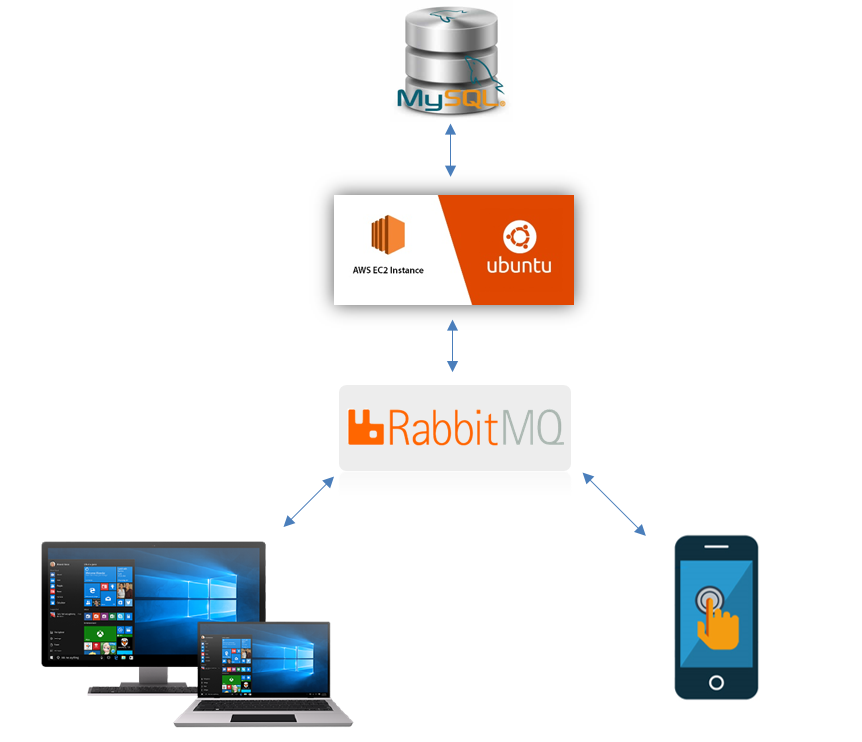
\includegraphics[width=0.8\textwidth]{img/rabbit.png}
	\caption{RabbitMQ e Database}
\end{figure}

\section{Implementation}
\subsection{Ashley Caselli}
\begin{itemize}
	\item Gradle configuration;
	\item Travis CI configuration;
	\item core: message interface and exceptions;
	\item organizer: mvc organization;
	\item organizer modelBroker: message sender/receiver;
	\item organizer javaFX;
	\item organizer grafic interface with Google Maps;
	\item server receiver: rabbitMQ connection and queue subscription;
\end{itemize}
\subsection{Carmine Vattimo}
\begin{itemize}
	\item server installation;
	\item database mySQL set-up;
	\item database operations crud;
	\item server receiver: database comunication for each kind of message;
	\item organizer Google Maps Markers;
\end{itemize}
\subsection{Francesca Tassinari}
\begin{itemize}
	\item player HTML;
\end{itemize}
\subsection{Giacomo Mambelli}
Nel progetto Treasure Hunt Organizer, Giacomo Mambelli si è occupato principalmente delle fasi di design e implementazione di:
\begin{itemize}
	\item Entità principali comuni a tutti i moduli software in collaborazione con AC
	\item Scambio dei messaggi in collaborazione con AC
	\item Applicazione mobile
\end{itemize}
\subsubsection{Applicazione mobile}
Il codice citato in questa sezione è contenuto nel package th-player.
L'applicazione è stata sviluppata come app ibrida, il framework utilizzato è Apache Cordova.
Tale software è attualmente fruibile tramite browser e android apk.

\subsubsection*{Login}
Alla prima apertura dell'applicazione l'utente viene guidato dall'interfaccia grafica nella creazione di un nuovo account il quale si concretizza in nome e password. Eseguita la registrazione, il login è automatico.
E' possibile effettuare il login, partendo dalla schermata principale della app, in un account precedentemente creato.
L'utente loggiato può fare logout cliccando sul nome utente che viene visualizzato nella bottom-bar della applicazione.
Per mantenere le informazioni sull'ultimo utente che ha effettuato l'accesso sono state utilizzate le local storage di HTML, che garantiscono la persistenza di piccole quantità di informazione sul device. Il logout comporta l'abbandono automatico della caccia al tesoro a cui l'utente sta partecipando (se esiste) con la relativa cancellazione dei dati persistenti; la rimozione di tutti i dati relativi all'utente salvati in fase di login.
Il controllo sulla validità dei dati inseriti nella form di login, così come il controllo sull'esistenza di un account con lo stesso username in fase di registrazione è stato implementato come scambio di messaggi con il server.

\subsubsection*{Mappa}
Per fornire precise informazioni al giocatore rispetto alla sua posizione si è deciso di incorporare una mappa all'interno della schermata di gioco.
La mappa scelta è quella di Google. Google Maps fornisce infatti API facilmente utilizzabili dalla maggior parte di sistemi software. In particolare è possibile richiamare le API Google tramite codice JavaScript importando uno script.
L'applicazione richiede pertanto le autorizzazioni necessarie per acquisire la posizione GPS del device. E stato necessario specificare nel file Manifest di Android l'utilizzo di tali dati da parte della app. L'utente dovrˆ accettare (in modo differente a seconda della piattaforma che utilizza) di fornire i dati relativi alla posizione per poter giocare correttamente.

\subsubsection*{Scambio Messaggi}
Lo scambio di messaggi con il server è stato realizzato sfruttando il middleware RabbitMQ.
Lato device è stato utilizzato il protocollo STOMP tramite WebSocket.
Il device apre una connessione al server al momento dell'avvio e ripristina la connessione ogni volta che essa viene persa.
Per evitare problemi di compatibilità con i vari browser si è deciso di aggiungere un ulteriore strato di WebSocket emulate con il plugin SockJ che è in grado di funzionare anche su browser che non supportano nativamente le WebSocket.
La connessione viene aperta dalla funzione connect() che imposta l'heartbeat a zero poichŽ non supportato dal plugin SockJS e successivamente contatta il server all'url specificato fornendo credenziali e callback.
I messaggi vengono inviati tramite una funzione denominata send() che comunica al server la queue alla quale è indirizzato il messaggio; una queue temporanea che viene creata al momento dell'invio tramite la quale ricevere la risposta ed il messaggio in formato testuale (Json) ricevuto in ingresso.
La funzione onReceive() è delegata alla ricezione dei messaggi sulla queue temporanea creata in fase di invio. Al suo interno il riconoscimento del tipo di messaggio basata sul campo messageType e la chiamata alla funzione corretta per la gestione dei vai tipi.
Tutti i messaggi sono in formato Json e devono pertanto essere deserializzati per poter essere sfruttati.
\begin{itemize}
	\item core: entities realizarion
	\item core: messages with serialization/deserialization;
	\item organizer: message exchange;
	\item server receiver: message recognizing and deserialization;
	\item player game logic in javascript, message exchange, data persist;
\end{itemize}
\subsection{Parti in comune}
\section{Deployment}
\section{Retrospection}
\begin{itemize}
	\item creare per i giocatori che parteciperanno a team un metodo per gestire loro più device che però si riferiscano al loro team;
	\item creare un messaggio che dopo un timer definito dall'organizzatore, che mandi dal device del team la sua posizione alla applicazione desktop per mostrare dove si trovano e l'organizzarore possa mandare un messaggio per aiutarli a trovare il prossimo punto di interesse;
	\item 
\end{itemize}
\vspace{-30pt}
\end{document}